\section{System architecture}

The paradigm choosen for our application is Client-Server. Each user will
connect to a remote server in order to use the application. The design model is
a three-tier application (Presentation, Middleware, Back-end), with a thin
client.

\begin{figure}[hpb]
	\centering
	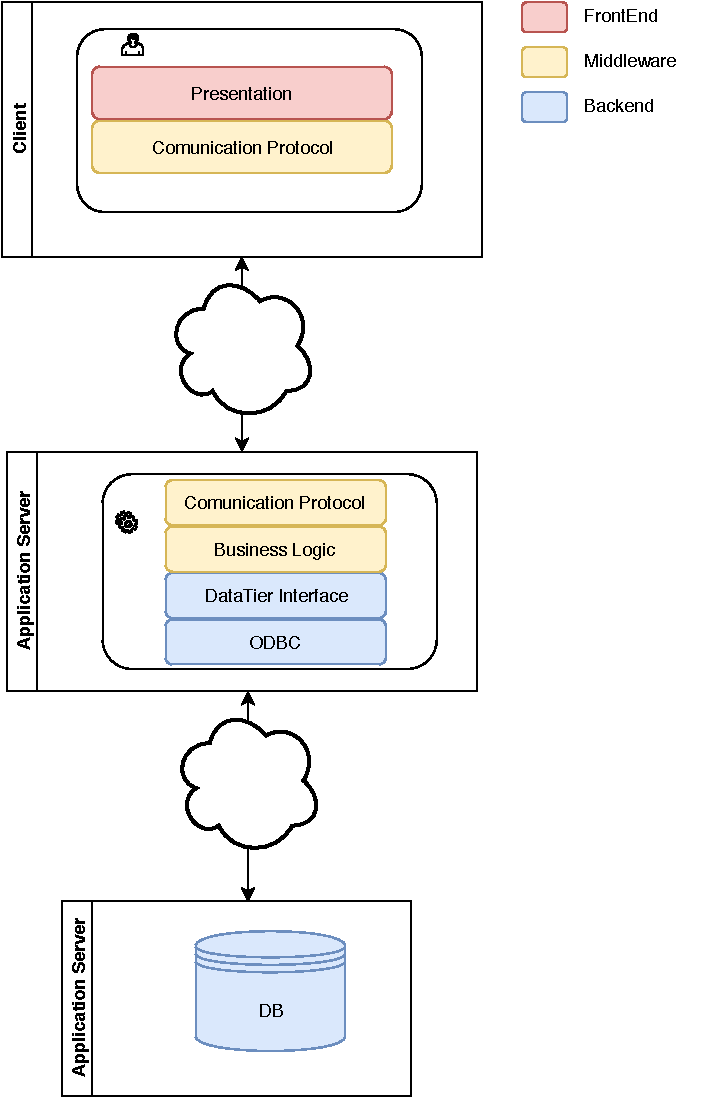
\includegraphics[width=\textwidth]{arch}
	\caption{System architecture diagram.}
	\label{fig:arch}
\end{figure}

The entire application will be developed in Java, following an object oriented
model. The DB used will be an SQL one, more precisely we will use MySQL.

\begin{description}
	\item[Client] The client part of the application is composed by two main
		components, a front end which manage the user interaction and a
		middleware that will handle the requests from the user and the
		response from the server side.
	\item[Server] The server part is, similarly to the client, divided in
		two parts: the middleware to handle the requests coming from the
		client side and a database manager, the back-end part, which
		will perform queries on the database.
\end{description}
